\documentclass{article}
\usepackage[hmargin=1in, vmargin=1in]{geometry}
\usepackage{makeidx}
\usepackage{fancyhdr}
\pagestyle{fancy}
\usepackage[pdftex]{graphicx}
\makeindex
\begin{document}
\begin{center}
\title{Three dimensional coordinates into two dimensional coordinates transformation}\\
\author{Edward Gerhold}
\city{Berlin, Germany}
\date{\today}
\maketitle

Version 0.1.9 (very drafty paper)\\

The formulas are correct.
The text itself is in the first stage.
And i have to learn \LaTeX{} for the first time.
Has to be overworked a few more times.

}\\
June 25, 2015\\
\end{center}

\texbf{Remark} On a piece of paper you see three coordinate axis pointing into three
directions in space. In reality these vectors are two dimensional. Because
they point into three directions on the paper, and not into the real space.\\

[[missing: Picture of a 3-D coordinate system with ijk-vectors on the axes pointing
into three directions. See \cite{Corral1} for introduction.]]\\

In this document we will design a basis for the coordinate transformation. A
basis is multiplied with the value of the coordinate to move to the correct new point.\\
In the case of cosines and sines, we move left and right and up and down, to 
tell you directly, what happens, when we multiply the coordinates with the matrix.\\

\section{Definitions}


\texbf{Definition} Let $\varphi_n$ be the set of axis angles, one for each axis. The angles start
at the same place, at the number zero. You have to arrange the $x$, $y$, and
$z$ axes like on a piece of paper around the unit circle by giving them the
appropriate angles. All three angles start at the default at zero. 

\begin{displaymath}
\varphi_n := \{\varphi_x, \varphi_y, \varphi_z\}
\end{displaymath}

\begin{example}
\texbf{Example}
The function rad converts degrees to radians, it´s useful for computer functions taking radians.
\begin{displaymath}
\text{rad}(\phi) := \frac{\pi}{180} \times \phi, \phi \in \mathbb{R}
\end{displaymath}
Here is an example of three angles. The three axes have an angle of 120 degrees beetween each.
\begin{displaymath}
\varphi_x = \text{rad 210},&&
\varphi_y = \text{rad 330},&&
\varphi_z = \text{rad 90} 
\end{displaymath}
\end{example}

\texbf{Definition} Let $e_n$ be the set of three two dimensional basis vectors, namely 
\vec{e}_x, $\vec{e}_y$ and $e_z$. Other names are $i$, $j$ or $k$ for example, like on the
picture of the coordinate system mentioned. The three vectors point into the three directions
of the three axes. On a piece of paper they are two dimensional, because they point into three
directions on the paper. The space being shown is what our brain completes, seeing three correct
axes. The three basis vectors represent exactly one unit into the direction of each axis. This
unit can be manipulated by multiplying the vector components inside $e_n$ with a factor $r_n$.

\begin{displaymath}
e_n := \{\vec{e}_x, \vec{e}_y, \vec{e}_z\}\\
\end{displaymath} 
 
This is the set of three basis vectors in set notation. To guess no numbers, it´s easier for us, 
for each vector, to go around the unit circle by the angles we already defined and to use cosine 
and sine for the correct $x$-distance and $y$-distance. For help, you should remember this parametrization 
of $x$ and $y$ from the unit circle. \footnote{Interested people can read about parametrization of x and y, 
the unit circle, polar coordinates and cosine and sine for example in the books \cite{Corral1}, \cite{Corral2}, \cite{Strang2}.}

\begin{displaymath}
\left(\begin{array}{1}x\\y\end{array}\right) = \left(\begin{array}{1}r \cos \varphi\\ r \sin \varphi\end{array}\right)\\
\end{displaymath}
\begin{displaymath}
(x,y) = (r \cos \varphi, r \sin \varphi)
\end{displaymath}

\begin{center}
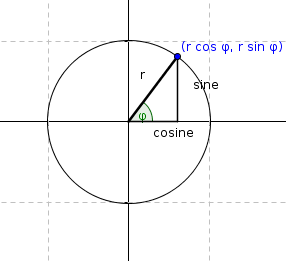
\includegraphics[scale=2]{unitcircle.png}
\end{center}

\texbf{Definition}

Modeling the three two dimensional basis vectors with this information,
we get the following three two dimensional basis vectors.\\

\begin{displaymath}
\vec{e}_x := (r_x\cos(\varphi_x), r_x\sin(\varphi_x) )^T = \left(\begin{array}{1}r_x\cos(\varphi_x)\\r_x\sin(\varphi_x) \end{array}\right)\\
\end{displaymath}
\begin{displaymath}
\vec{e}_y := (r_y\cos(\varphi_y), r_y\sin(\varphi_y) )^T = \left(\begin{array}{1}r_y\cos(\varphi_y)\\r_y\sin(\varphi_y) \end{array}\right)\\
\end{displaymath}
\begin{displaymath}
\vec{e}_z := (r_z\cos(\varphi_z), r_z\sin(\varphi_z) )^T = \left(\begin{array}{1}r_z\cos(\varphi_z)\\r_z\sin(\varphi_z) \end{array}\right)\\
\end{displaymath}

One for each component of $(x,y,z)$ By multiplying with, we move the 
points into the right pieces of direction. On the plane we use to point into three directions.\\

\begin{center}
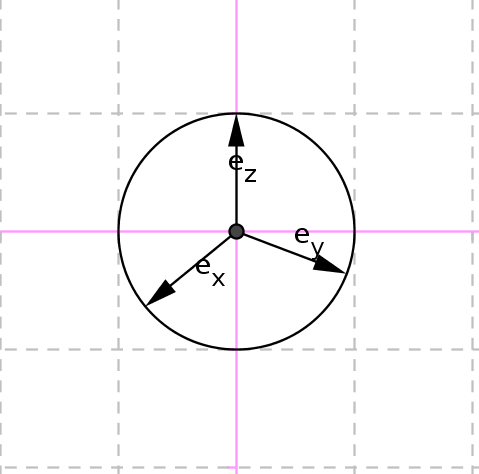
\includegraphics[scale=1]{unitvectors.png}
\end{center}

\texbf{Remark}.The values of $r_x, r_y$ and $r_z$ decide, how long one unit into each
direction is. To preserve affine graphical transformations all three
axes should have the same length, to represent same distance for each coordinate unit, 
which can generally be enlarged or made smaller than \emph{unit length}, which is a length of $1$. 
By default the resulting vector of the cosine and sine Components has \emph{unit length}, 
if you don´t multiply the cosine and the sine with $r_x, r_y$ and $r_z$ in each basis vector. \\

\texbf{Remark} On the other side, the length of $r$ can be determined from existing basis vectors, 
by pulling the square root out of the sum of the squares of the vector components.
This is also known as euclidean norm, or the root of the inner product of the vector with itself.
Like real fans of sines and cosines, we know that $\sin^2 \varphi + \cos^2 \varphi = 1$ and what the root of 1 is.
If we pull the root out of the products of cosine and sine multiplied with $r \ne 1$ , we get the length of $r$ again. 
$r = \sqrt{\vec{x} \dotproduct \vec{x}}$ = $\left(\Sigma_{i=1}^{n} \vec{x}_i^2\right)^{\frac{1}{2}}$.\\


Now about the multiplication of the coordinates with the basis.\\

\emph{The other help we take} The other lemma we need is the theorem for 
multiplying with the orthogonal basis.\\

In our case the 90°-orthogonality rules don´t count, we arrange for example with about 120° beetween each around the origin on a plane. The point is, the generic formula still holds.\\

\texbf{Remark} The sum of the basis multiplied with the coordinates is nothing
new. But literature and lecture scripts just tell how to multiply
same dimensions, giving no clue about the easy 3-D to 2-D conversions.
I can not speak for all, and do not believe, that no one told no one about this, 
but i have not met any one in the last twenty years telling me about this easy 
transformation and computer graphics went another, more complicated way, over
homogeneous coordinates, 4 by 4 matrices and a final viewport division, to get
the points back to two dimensions.\\

The formula for multiplying a vector with a base to get a new vector is this. \\

\begin{displaymath}
\vec{v} = \displaystyle\sum_{i=1}^{n} \vec{x}_i\vec{e}_i
\end{displaymath}

It is done componentwise for each row of the vector.\\
With $\vec{x}_i$ as the coordinate components and $\vec{e}_i$ as the corresponding basis vector component and $\vec{v}$ as the resulting new vector.\\

This is also equal to

\begin{displaymath}
\vec{v} = x\vec{i} + y\vec{j} + z\vec{k}
\end{displaymath}

what also explains, what the ijk-Notation means. If you don´t use it already for determining determinants for
calculating cross products. It´s for describing a vector. Don´t forget, our $i, j, k$ basis is two dimensional, 
because we draw on a 2-D plane like the computer screen or a piece of paper. \\

With a 3x3 basis the vector $x\vec{i} + y\vec{j} + z\vec{k}$ is equal to \left(\begin{array}{1}x'\\y'\\z'\end{array}\right)$. But with a 2x3 basis the vector $x\vec{i} + y\vec{j} + z\vec{k}$ is becoming  \left(\begin{array}{1}x'\\y'\end{array}\right)$\\

Finishing the matrix\\

Each $(x,y,z)$ coordinate has to be multiplied for the new $(x',y')$
with it´s corresponding term of the basis vectors in the matrix. That means,
to sum the products with $(x,y,z)$ and the cos terms up for $x'$ and to sum the products
of $(x,y,z)$ and the sin terms up for $y'$. This is the same as imagining walking left and
right with $\cos \varphi$ and up and down with $\sin \varphi$. Or mathematically adding positive or negative values.\\

\begin{displaymath}
\left(\begin{array}{1}x'\\y'\end{array}\right) = \left(\begin{array}{1}
xr_x\cos(\varphi_x) + yr_y\cos(\varphi_y) + zr_z\cos(\varphi_z)\\
xr_x\sin(\varphi_x) + yr_y\sin(\varphi_y) + zr_z\sin(\varphi_z)\end{array}\right)\\
\end{displaymath}

\section{Theorem}
\index{Definition}
\newtheorem{Definition}{Definition}
\begin{Definition}
Let \boldsymbol{A} be the matrix containing the three two dimensional unit vectors in order, one each
column. You get a 2x3 matrix\footnote{A 2x3 Matrix, which i proudly gave the nickname
Gerhold Projection Matrix to distinguish it from other matrices, making sure it contains the three two dimensional and trigonometric basis vectors, which allow arranging the projection vectors just by going around the circle instead of guessing wild numbers.
} $\boldsymbol{A} \in \mathbb{R}^{2x3}: \mathbb{R}^{3} \rightarrow \mathbb{R}^{2}$. With the basis vectors $\left(\begin{array}{1}r_n \cos \varphi_n\\r_n \sin \varphi_n\end{array}\right)$ in the three columns. 

\begin{displaymath}
\boldsymbol{A} := \left(
    \begin{array}{111}\vec{e}_x & \vec{e}_y & \vec{e}_z
    \end{array}\right)
    = \left(
    \begin{array}{111}
    r_x\cos(\varphi_x) & r_y\cos(\varphi_y) & r_z\cos(\varphi_z) \\
    r_x\sin(\varphi_x) & r_y\sin(\varphi_y) & r_z\sin(\varphi_z) \\
    \end{array}
\right)\\
\end{displaymath}
\end{Definition}

\index{Theorem}
\newtheorem{Theorem}{Theorem (The Fundamental Theorem of transforming 3-D Points into 2-D Points)}
\begin{Theorem} \emph{}:\\

If you multiply  \boldsymbol{A}, the matrix of the three two-dimensional unit vectors,
with the three-coordinate points $(x,y,z)$, the result is a two coordinate point, 
$(x',y')$. This point $(x',y')$ is the correct point on the two dimensional plane,
representing the point from the three dimensional coordinate system, you are transforming.\\

\begin{displaymath}
\boldsymbol{A}\left(\begin{array}{1}x\\y\\z\end{array}\right) = \left(\begin{array}{1}x'\\y'\end{array}\right)
\end{displaymath}

Applying the operator\footnote{The \emph{Gerholdian projection operator} is my favorite nickname for this matrix} performs the following operation\\

\begin{equation}
\begin{displaymath}
\boldsymbol{A}\left(\begin{array}{1}x\\y\\z\end{array}\right) = x\vec{e}_x + y\vec{e}_y + z\vec{e}_z\\
\end{displaymath}
\begin{displaymath}
&= \left(\begin{array}{1}xr_x\cos(\varphi_x) + yr_y\cos(\varphi_y) + zr_z\cos(\varphi_z)\\
xr_x\sin(\varphi_x) + yr_y\sin(\varphi_y) + zr_z\sin(\varphi_z)\\
\end{array}\right) = \left(\begin{array}{1}x'\\y'\end{array}\right)
\end{displaymath}
\end{equation}

\end{Theorem}

\texbf{Proof}\\
\begin{displaymath}
\boldsymbol{A}\left(\begin{array}{1}x\\y\\z\end{array}\right) = x\vec{e}_x + y\vec{e}_y + z\vec{e}_z = \left(\begin{array}{1}x'\\y'\end{array}\right)
\end{displaymath}

\begin{displaymath}
\left(\begin{array}{1}x'\\y'\end{array}\right) = \left(\begin{array}{1}
xr_x\cos(\varphi_x) + yr_y\cos(\varphi_y) + zr_z\cos(\varphi_z)\\
xr_x\sin(\varphi_x) + yr_y\sin(\varphi_y) + zr_z\sin(\varphi_z)\end{array}\right)
\end{displaymath}\\

\texbf{Example}\\
The following is example code for varius computer systems.\\
$x\_ = x*r*cos(alpha) + y*r*cos(beta) + z*r*cos(gamma)\\
y\_ = x*r*sin(alpha) + y*r*sin(beta) + z*r*sin(gamma)$\\

\texbf{Example}\\
\begin{example}
The following is an EcmaScript 6 Arrow Function returning the new point. It is not optimized for speed. Means, to repeat the sin and cosine calls.\\
\texbf{Example for Programmers}
\mbox\parbox{ let projection = ([x,y,z]) =\rangle [x*r*Math.cos(xAxisAngle) + y*r*Math.cos(yAxisAngle) + z*r*Math.cos(zAxisAngle),x*r*Math.sin(xAxisAngle) + y*r*Math.sin(yAxisAngle) + z*r*Math.sin(zAxisAngle)]; 
}
}
\end{example}

\section{Corollary}

The theorem can be extended into more dimension to go down to any other dimension.
The generic case is known to linear algebra, i found it lately after beginning this
document and will include the information within the next versions.\\

\texbf{Corollary} \emph{(Converting any Dimensions down to less dimensions)}:\\

The theorem can be extended to more dimensions, for example can four two-dimensional
vectors represent a 4-D space on the 2-D plane. They get converted into the correct
 2-D points. For Example, if you use a 2x4 matrix and convert all points at each 
instance of $t$ you have a moving object into the direction of the fourth basis vector. \\

\begin{displaymath}
\boldsymbol{A} := \left(
    \begin{array}{1111}\vec{e}_x & \vec{e}_y & \vec{e}_z & \vec{e}_t\end{array}\right)\\ = \left(
    \begin{array}{1111}
    r_x\cos(\varphi_x) & r_y\cos(\varphi_y) & r_z\cos(\varphi_z) & r_t\cos(\varphi_t)\\
    r_x\sin(\varphi_x) & r_y\sin(\varphi_y) & r_z\sin(\varphi_z) & r_t\sin(\varphi_t)\\
    \end{array}
\right)
\end{displaymath}

Here the basis is four times of two dimensions. A 2x4 matrix. 

\begin{displaymath}
\boldsymbol{A}\left(\begin{array}{1}x\\y\\z\\t\end{array}\right) = \sum_{n} \vec{e}_n\vec{x}_n = \left(\begin{array}{1}x'\\y'\end{array}\right)\\
\end{displaymath}

\texbf{Proof}:

\begin{displaymath}
\boldsymbol{A}\left(\begin{array}{1}x\\y\\z\\t\end{array}\right) &= \left(\begin{array}{1}
xr_x\cos(\varphi_x) + yr_y\cos(\varphi_y) + zr_z\cos(\varphi_z) + zr_t\cos(\varphi_t)\\
xr_x\sin(\varphi_x) + yr_y\sin(\varphi_y) + zr_z\sin(\varphi_z)+ zr_t\sin(\varphi_t)\end{array}\right)\\
\end{displaymath}
\begin{displaymath}
&= x\vec{e}_x + y\vec{e}_y + z\vec{e}_z + t\vec{e}_t &= \sum_{n} \vec{e}_n\vec{x}_n &= \left(\begin{array}{1}x'\\y'\end{array}\right)
\end{displaymath}

The same method can be used to convert any other number of dimensions to the $xy$-plane. But it can also be
used in a generic m by n case\footnote{http://de.wikipedia.org/wiki/Abbildungsmatrix, also found in lecture scripts, but not anyone explaining me this matrix here or the topic of the from-three-to-two-points conversion. Is it too obvious? Or isn´t it obvious?}, to convert from n dimension down to m, if you know the basis for the destination.

\section{Summary}

\texbf{Summary of all neccessary steps}
\begin{enumerate}
\item Lay out the three basis vectors around a circle and write down the angles $\varphi_n$. Programmers have to write down a variable for anyways.
\item Write down the basis vectors $\vec{e}_n$ as $r_n \cos \varphi_n$ and $r_n \sin \varphi_n$ (two dimensional). Don´t multiply with $r_n$ for a unit length of $1$ or multiply with $r_n$ to change the length of the basis vector.
\item Put the three basis vectors $\vec{e}_n$ into a matrix \bigsymbol{A}. Programmers can directly code the two lines of multiplication and forget the formal rest.
\item Iterate over your points and multiply each $(x,y,z)$ with the matrix \boldsymbol{A}, which acts as our linear operator, and put $(x',y')$ into your new set.
\end{enumerate}

\texbf{Remark}\\
About the word \emph{unit}. I am not really sure, if i have to use \emph{base vector} for a vector of any length and \emph{unit vector} only for the \emph{unit length} of $1$. Because of the misleading mismatch with the \emph{unit} of the thought \emph{coordinate axes}, which the \emph{base vector} defines, i tend in the first versions to misuse the word \emph{unit vector} for both. If you find this, or any other formal mistake, be sure, it is not wanted :-) I will try to remove more of these spelling errors in the next versions.

\begin{thebibliography}    

    \bibitem{Corral1} \textit{Michael Corral, Schoolcraft College},
		    Vector Calculus, GNU Free Documentation License, http://mecmath.net 
    \bibitem{Corral2} \textit{Michael Corral, Schoolcraft College},
		    Trigonometry, GNU Free Documentation License, http://mecmath.net         
    \bibitem{Strang1} \textit{Gilbert Strang, MIT},
		    Linear Algebra and it´s Applications. Fourth Edition.
    \bibitem{Strang2} \textit{Gilbert Strang, MIT},
            Calculus. MIT OpenCourseWare Supplemental Resources. http://ocw.mit.edu    
    \bibitem{Corral3} \textit{Michael Corral, Schoolcraft College},
            Latex Mini Tutorial, http://mecmath.net            
    \bibitem{Jürgens,Feuerstack} \textit{Manuela J\"urgens, Thomas Feuerstack},
            LaTeX, eine Einf\"uhrung und ein bisschen mehr..., Fernuniversit\"at Hagen, a026\_latex\_einf.pdf
    \bibitem{Rudl} \textit{Dr.Jan Rudl},
            Einf\"uhrung in LaTeX, Technische Universit\"at Dresden, Fachbereich Mathematik, LaTeX-Kurs.pdf            

\end{thebibliography}
\printindex
\end{document}